\section{Method}

We wish to verify the viability of RRC systems.
This requres us to be able to reproduce at least some previously published results.
Therefore, we will create a functioning RRC system, as in \cite{rbn-reservoir},
and test it on the datasets presented in the same paper.
We will also re-use the computational capability measure introduced there,
and see if the relationship between it and accuracy can be recreated.

Secondly, we wish to test the effectiveness of creating new RBN rervoirs for existing readout layers through artificial evolution.
If this is found to be the case, it would imply a many-to-one correspondence between RBN-reservoirs and readout layers.
These sets of re-useable  reservoirs must necessarily have some similar characteristics,
to allow our re-use of the readout layer to make sense.
We will attempt to find any similarities there might be.
In addition, such a finding can shed light on the optimal genome representation to use for evolving RBN reservoirs.

The following systems have been implemented to investigate the stated questions.

\begin{itemize}
  \item An RBN simulator
  \item Procedures for analyzing and visualizing RBNs
  \item Procedures for creating classification tasks

  \item An RBN-Reservoir Computing system using:
  \begin{itemize}
    \item The forementioned RBN simulator as a reservoir
    \item The ridge regression node from the Oger RC toolkit \cite{verstraeten2012oger} as readout layer
    \item The Python Modular toolkit for Data Processing \cite{zito2008modular} for glue and training of the RRC system.
  \end{itemize}
  \item A system for evolving RBNs given certain constraints, using a genetic algorithm based on the one used in \cite{farstad2015evolving}.
\end{itemize}

The codebase is available on GitHub \cite{forprosjekt-code-github} under a soon-to-be permissive licence.

\subsection{Measuring computational capability}

We will be using the computational complexity measure introduced in \ref{section:computational-capability} to analyze the created RBNs.
This measure is parameterized over both input stream length $T$ and the required depth of separation $t$.
To make this an useful measure when comparing against reservoir accuracy on a specific task,
we will chose values of $T$ similar to the length and $t$ equal to the required memory of that task.

\subsection{The creation and training of a functioning RRC system}

The final RRC system is shown as a block diagram in \ref{figure:rrc-block},
and the actual network topology is equivalent as the one in figure \ref{figure:rbn-reservoir}.

\begin{figure}
  \centering
  \begin{tikzpicture}
    \node (dataset) {Dataset};
    \node[box, below=of dataset] (input) {Input layer};
    \node[box, right=of input] (reservoir) {RBN Reservoir};
    \node[box, right=of reservoir] (readout) {Readout layer};
    \node[above=of readout] (classification) {Classification};

    \node[draw,dotted,fit=(input) (reservoir) (readout), label={RRC}] {};

    \draw[edge] (dataset) to (input);
    \draw[edge] (input) to (reservoir);
    \draw[edge] (reservoir) to (readout);
    \draw[edge] (readout) to (classification);
  \end{tikzpicture}
  \caption{Block diagram of the RRC processing a dataset.}
  \label{figure:rrc-block}
\end{figure}

\subsubsection{testing}

To verify that RBN simulation is working,
a RBN is created randomly, initial state set to all zeros, and ran.
The results are visualized in figure \ref{figure:rbn-noperturb}.
We see that the RBN exhibits stable dynamics, and enters into an attractor around $t=15$.
In figure \ref{figure:rbn-perturb} we continiously perturb the RBN with the input stream from the Temporal Parity task visualized in \ref{figure:temporal-parity}.
In the perturbed case, the state trajectory is continiously changed, preventing the RBN from settling into an attractor.
Interestingly enough, there seems to be a visual similarity between the two cases.
Such a pattern is sure to dissapear with a RBN in the chaotic phase.

This erratic pattern of state transitions is then fed into the readout layer,
which is then tasked with finding a linear combination of the RBN states that results in the expected output for the given task.

\begin{figure}
  \subfloat[Unperturbed]{
    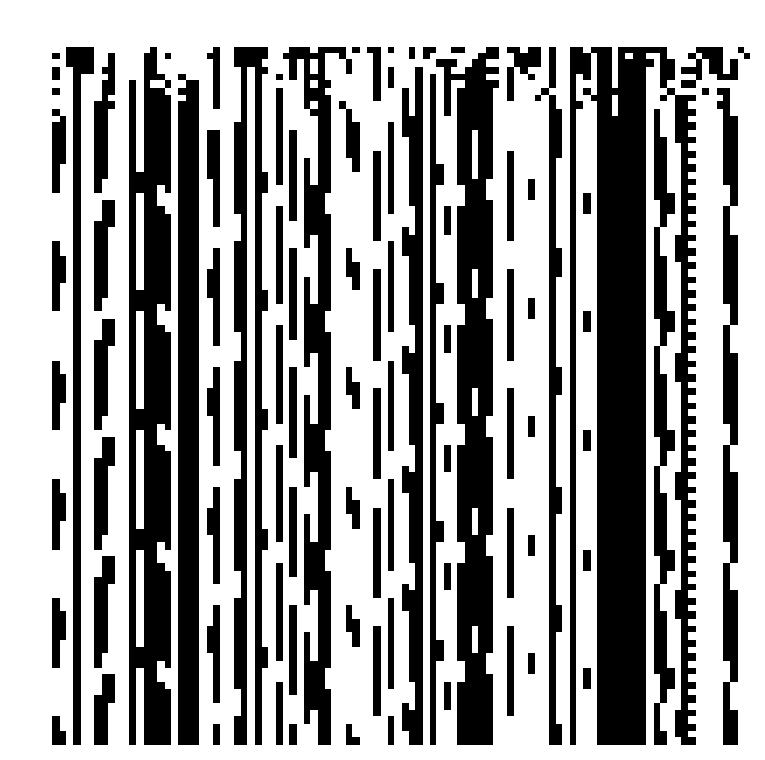
\includegraphics[width=0.5\columnwidth]{method/final-1-noperturb.pdf}
    \label{figure:rbn-noperturb}
  }
  \subfloat[Perturbed]{
    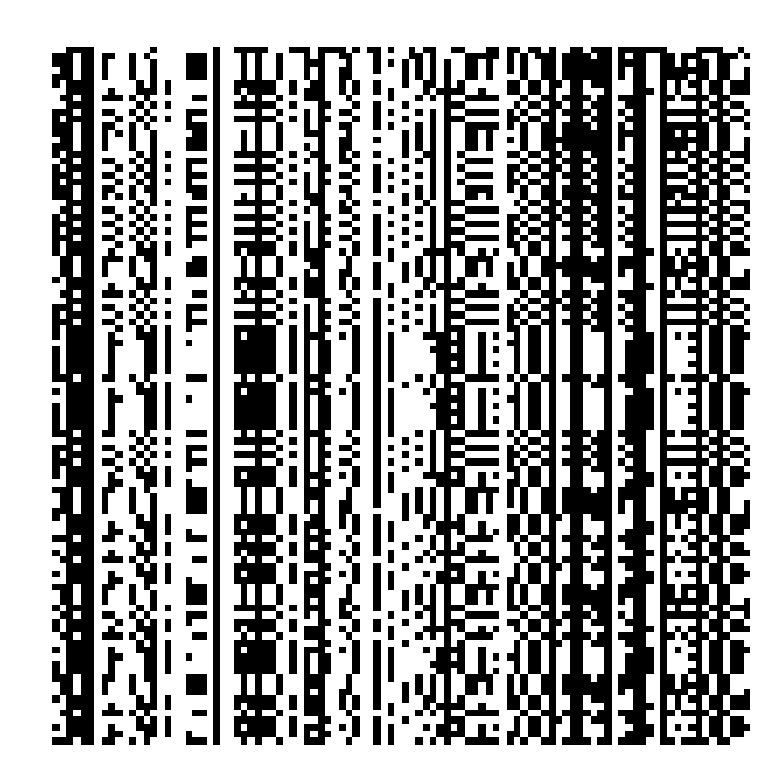
\includegraphics[width=0.5\columnwidth]{method/final-1-perturb.pdf}
    \label{figure:rbn-perturb}
  }
  \caption{
    The same RBN ($N=100, K=2, P=0.5, L=50$) shown both perturbed and unperturbed.
    The boolean states of the RBN are plotted along the X-axis,
    with time flowing downwards.
  }
\end{figure}

\subsubsection{training}

The training process for a RRC system is threefold.

First, we create a number of datasets for training,
as well as a dataset for later testing.
These datasets are either Temporal Parity or Density,
as described in section \ref{subsection:rbn-reservoir-systems}.

We then either create a new RBN (initialize it randomly),
or load a previously created RBN from disk.

For each bit of input in each dataset,
we perturb the input-connected nodes in the RBN.
After each perturbance, the RBN is ran synchronously (CRBN mode) for one timestep.
The resulting RBN states are collected,
and after the entire dataset is processed,
forwarded to the readout layer.

To find a suitable mapping from the set of reservoir states and the correct input classification,
ridge regression \cite{hoerl1970ridge} is used.
This version of least squares regression is more accurate when faced with input colinearities,
as well as always being at least as accurate as ordinary least squares.

This process is repeated for all the datasets,
and the final regression parameters are chosen as a combination of the parameters obtained for each individual dataset.
Finally we measure the normalized accuracy of the trained reservoir on the test dataset,
defined as
\begin{equation}
Accuracy = 1 - \dfrac{sum(actual\_output \neq expected\_output)}{len(correct\_output)}
\label{formula:accuracy}
\end{equation}
.
If the RRC system achieves a high accuracy on an interesting task,
it will be stored for further research.

\subsection{The evolving of functionally equivalent RBN reservoirs for existing readout layers}
\label{section:method:evolving-rbns}

To investigate the potential many-to-one mapping between RBN-reservoirs and readout layers,
we'll be using a genetic algorithm (as presented in section \ref{section:background:ga}) to evolve candidate RBNs,
using a fixed test dataset and readout layer for fitness evaluation.

\subsubsection{Genotype and phenotype representation}

We let the genotype be a direct encoding of the corresponding RBN graph.
Such an encoding is significantly larger than a generative encoding,
but less complex as well as able to generate all individuals in the fitness landscape.

Each node needs to represent whether it is connected to the input node,
who its neighbors are, and what its transition rule is.
As we only look at homogenous RBNs,
we can use a fixed-length genome with
\begin{equation}
genome\_length = n\_nodes \cdot (connectivity + 2)
\end{equation}
To further simplify GA implementation,
we let all symbols in the genome take a value in the range $[0, max\_required\_in\_genome)$.
The actual symbol values are then computed modulo the largest actual value they could take on
(2 for input connectivity, n\_nodes for neighbors, $2^{2^{n\_nodes}}$ for transition rules).
This redundancy in the genome can be an advantage,
as it allows for new ways to explore the fitness landscape \cm.

The final genome is shown in figure \ref{figure:rbn-genotype}.
Note that this representation sets no limitations on input connectivity or uniqueness of neighbors.

\begin{figure}
  \centering
  \begin{bytefield}[bitwidth=1.5em]{12}
    \bitheader{0-11} \\
    \bitbox{1}{C} \bitbox{1}{N\textsubscript{1}} \bitbox{1}{N\textsubscript{2}} \bitbox{1}{R}
    \bitbox{1}{C} \bitbox{1}{N\textsubscript{1}} \bitbox{1}{N\textsubscript{2}} \bitbox{1}{R}
    \bitbox{1}{C} \bitbox{1}{N\textsubscript{1}} \bitbox{1}{N\textsubscript{2}} \bitbox{1}{R} \\
    \bitbox[t]{4}{$\underbrace{\hspace{6em}}_{\text{\normalsize Node 1}}$}
    \bitbox[t]{4}{$\underbrace{\hspace{6em}}_{\text{\normalsize Node 2}}$}
    \bitbox[t]{4}{$\underbrace{\hspace{6em}}_{\text{\normalsize Node 3}}$} \\
  \end{bytefield}
  \caption{
    The direct-encoded genotype used for evolving RBNs,
    shown here for an RBN with $N=3, K=2$.}
  \label{figure:rbn-genotype}
\end{figure}

\subsubsection{Fitness function}

Each GA run is parameterized with an already-trained and accurate readout layer (separated from its RBN-reservoir),
as well as a single test dataset of the same origins as the dataset used for training the readout layer.
After converting each genotype to its corresponding phenotype,
the resulting RBN is connected to the readout-layer and fed with the fixed test dataset.
The accuracy obtained,
as calculated in formula \ref{formula:accuracy},
is used as the fitness of the phenotype.

\subsubsection{GA hyperparameters}

The hyperparameters for the GA are presented in table \ref{table:ga-hyperparameters}.

\begin{table}
  \centering
  \caption{GA hyperparameters}
  \label{table:ga-hyperparameters}
  \begin{tabular}{ll}
    Children pool size             & 40                                    \\
    Adult pool size                & 40                                    \\
    Fitness satisfaction threshold & 0.98                                  \\
    maximum generations            & 200                                   \\
    Adult selection                & Generational mixing                   \\
    Parent selection               & Tournament selection(K=8)             \\
    Genome crossover               & Per component crossover (p=0.5)       \\
    Genome mutation                & Per genome component mutation (p=0.1) \\
  \end{tabular}
\end{table}

Adult selection is simple generational mixing,
selecting the best 40 specimens from the combined children and adult populations.
Per component crossover will with a probability p either pass through the entire genome from the left parent,
or for each component chose either the left or right parents value with a probability 0.5.
Per genome component mutation will reroll each genome component with probability p.
This value is set relatively high (0.1) due to experiments showing a much faster convergence rate fr this domain than with the initial chosen value of 0.01.
